\section{Kritische Punkte}
\label{sec:kritischePunkte}

Zur Erinnerung: Bei einer Funktion in einer Variablen kann man die Extremalpunkte leicht wie folgt finden:
\begin{enumerate}
	\item Man ermittelt die sogenannten kritischen Stellen. Das sind jene Stellen, in denen der Graph eine horizontale Tangente aufweist, und entsprechen somit den Nullstellen der Ableitung.
	\item Die Art des Punktes kann mit der zweiten Ableitung ermittelt werden: Ist die zweite Ableitung an einer kritischen Stelle positiv, so liegt ein lokales Minimum vor. Falls die zweite Ableitung negativ ist, befindet sich an der entsprechenden Stelle ein lokales Maximum.
\end{enumerate}
Auf den folgenden Seiten werden wir ähnliche Kriterien für Funktionen in zwei Variablen erarbeiten.

\subsection{Kritische Punkte}

Die kritischen Punkte sind im Falle von Funktionen in zwei Variablen jene Punkte, in denen die Tangentialebene an den Graphen parallel zur $xy$-Ebene verläuft.
\begin{center}
	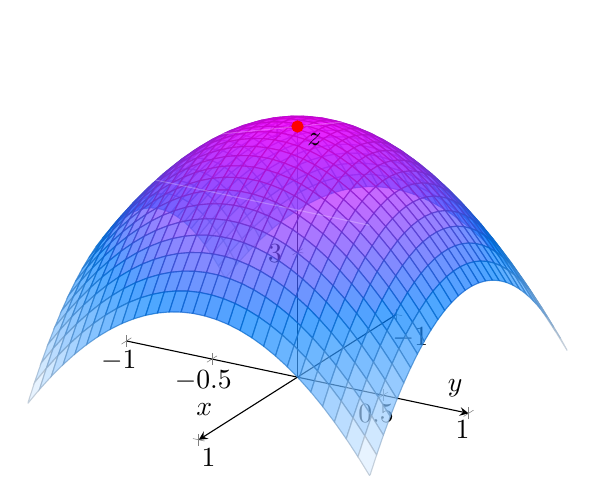
\begin{tikzpicture}
		\begin{axis}[
				view={120}{30},
				axis lines=center,
				xlabel={$x$},
				ylabel={$y$},
				zlabel={$z$},
				domain=-1:1,
				y domain=-1:1,
				samples=30,
				colormap/cool,
			]
			% Surface plot (flipped to represent a maximum)
			\addplot3[surf, opacity=0.7] {-x^2 - y^2 + 4};

			% Tangent plane at the maximum
			\addplot3[surf, opacity=0.25, colormap/blackwhite]
			coordinates {
					(-1, -1, 4) (-1, 1, 4) (1, -1, 4) (1, 1, 4)
				};

			% Critical point (maximum)
			\addplot3[mark=*, color=red] coordinates {(0, 0, 4)};
		\end{axis}
	\end{tikzpicture}
\end{center}

Unter den kritischen Punkten unterscheidet man grob drei Arten: lokale Maxima, lokale Minima und Sattelpunkte.

\begin{center}
	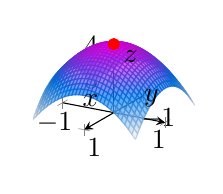
\begin{tikzpicture}
		\begin{axis}[
				view={120}{30},
				axis lines=center,
				xlabel={$x$},
				ylabel={$y$},
				zlabel={$z$},
				domain=-1:1,
				y domain=-1:1,
				samples=30,
				colormap/cool,
				width=0.3\textwidth,
			]
			% Maximum
			\addplot3[surf, opacity=0.7] {-x^2 - y^2 + 4};
			\addplot3[mark=*, color=red] coordinates {(0, 0, 4)};
		\end{axis}
	\end{tikzpicture}
	\hfill
	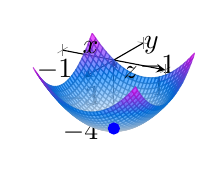
\begin{tikzpicture}
		\begin{axis}[
				view={120}{30},
				axis lines=center,
				xlabel={$x$},
				ylabel={$y$},
				zlabel={$z$},
				domain=-1:1,
				y domain=-1:1,
				samples=30,
				colormap/cool,
				width=0.3\textwidth,
			]
			% Minimum
			\addplot3[surf, opacity=0.7] {x^2 + y^2 - 4};
			\addplot3[mark=*, color=blue] coordinates {(0, 0, -4)};
		\end{axis}
	\end{tikzpicture}
	\hfill
	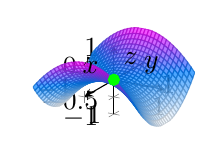
\begin{tikzpicture}
		\begin{axis}[
				view={120}{30},
				axis lines=center,
				xlabel={$x$},
				ylabel={$y$},
				zlabel={$z$},
				domain=-1:1,
				y domain=-1:1,
				samples=30,
				colormap/cool,
				width=0.3\textwidth,
			]
			% Saddle point
			\addplot3[surf, opacity=0.7] {x^2 - y^2};
			\addplot3[mark=*, color=green] coordinates {(0, 0, 0)};
		\end{axis}
	\end{tikzpicture}
\end{center}

Da die Tangentialebene in diesen Punkten horizontal verläuft, hat sie eine Gleichung der Form
\[
	z = c
\]
Das heisst, dass in der Gleichung die Variablen \(x\) und \(y\) nicht vorkommen, bzw. dass deren Koeffizienten Null sind. Allgemein haben aber Tangentialebenen an den Graphen einer Funktion \(f\) an der Stelle \((x_0, y_0)\) die Gleichung
\[
	z = f(x_0, y_0) + \frac{\partial f}{\partial x}(x_0, y_0) \cdot (x - x_0) + \frac{\partial f}{\partial y}(x_0, y_0) \cdot (y - y_0)
\]
Die Koeffizienten von \(x\) und \(y\) sind im Allgemeinen also \(\frac{\partial f}{\partial x}(x_0, y_0)\) und \(\frac{\partial f}{\partial y}(x_0, y_0)\). Die Tangentialebene \(f\) an der Stelle \((x_0, y_0)\) verläuft also genau dann parallel zur \(xy\)-Ebene, wenn
\[
	\frac{\partial f}{\partial x}(x_0, y_0) = 0 \quad \text{und} \quad \frac{\partial f}{\partial y}(x_0, y_0) = 0
\]
ist.


\begin{definition}
	{Kritische Stellen}{}
	Die kritischen Stellen einer Funktion \(f(x, y)\) sind jene Stellen \((x_0, y_0)\), für welche gilt:
	\[
		\vec{\nabla} f(x_0, y_0) = \vec{0}
	\]
\end{definition}

\begin{bsp}
	{}{}
	$$f(x,y)=x^2+xy-y$$
	\vspace*{8cm}
\end{bsp}
\clearpage
\begin{bsp}
	{}{kritischePunkte2}
	$$f(x,y)=x^3+xy^2-x$$
	\vspace*{15cm}
\end{bsp}

\begin{ueb}
	{}{}
	\begin{enumerate}
		\item Bestimmen Sie die kritischen Stellen der folgenden Funktionen und zeichnen Sie deren Graphen mit Geogebra:
		      \begin{enumerate}
			      \item \(f(x,y) = -10x + 2xy + y^3\)
			      \item \(f(x,y) = x^2y - x^2 - y^2\)
			      \item \(f(x,y) = e^{x^2 + 4x + y^2}\)
		      \end{enumerate}
	\end{enumerate}
\end{ueb}

\clearpage
\emph{Lösungen}
\begin{enumerate}
	\item \(K = \left(-\frac{75}{2}, 5\right)\)
	\item \(K_1 = (0, 0), \, K_2 = \left(\sqrt{2}, 1\right), \, K_3 = \left(-\sqrt{2}, 1\right)\)
	\item \(K = (-2, 0)\)
\end{enumerate}

















\clearpage
\subsection{Hesse-Matrix}
\label{sec:hesseMatrix}
Im letzten Kapitel haben Sie eine Methode kennengelernt, wie man die kritischen Punkte einer Funktion finden kann. Allerdings bleibt noch die Frage, ob es sich dabei um lokale Minima, Maxima oder Sattelpunkte handelt. Wie bei Funktionen in einer Variablen werden wir dazu die zweite Ableitung betrachten. Davon gibt es aber mehrere!

Betrachten wir die Funktion \(f(x,y) = x^2 + 2xy^2 + y^3\). Die partielle Ableitung in Richtung der \(x\)-Achse lautet
\[
	\frac{\partial f}{\partial x}(x,y) = 2x + 2y^2.
\]
Formal ist diese partielle Ableitung wieder eine Funktion in zwei Variablen und kann nochmals partiell abgeleitet werden. Die partielle Ableitung von \(\frac{\partial f}{\partial x}\) in \(x\)-Richtung ist dann:
\[
	\frac{\partial^2 f}{\partial x^2}(x,y) = 2.
\]
Die partielle Ableitung von \(\frac{\partial f}{\partial x}\) in \(y\)-Richtung ist dagegen:
\[
	\frac{\partial^2 f}{\partial y \partial x}(x,y) = 4y.
\]
Analog kann auch \(\frac{\partial f}{\partial y}(x,y) = 4xy + 3y^2\) erneut nach \(x\) oder \(y\) abgeleitet werden, und es entstehen die zweifachen partiellen Ableitungen:
\[
	\frac{\partial^2 f}{\partial x \partial y}(x,y) = 4y, \quad \frac{\partial^2 f}{\partial y^2}(x,y) = 4x + 6y.
\]


\begin{definition}
	{Partielle Ableitung zweiter Ordnung}{}

	Sind die partiellen Ableitungen einer Funktion selbst wieder partiell differenzierbar, so nennt man die Funktionen
	\[
		\frac{\partial^2 f}{\partial x^2}(x,y) = \frac{\partial}{\partial x} \left( \frac{\partial}{\partial x} f(x,y) \right), \quad
		\frac{\partial^2 f}{\partial y \partial x}(x,y) =\frac{\partial}{\partial y} \left( \frac{\partial}{\partial x} f(x,y) \right),
	\]
	\[
		\frac{\partial^2 f}{\partial x \partial y}(x,y)= \frac{\partial}{\partial x} \left( \frac{\partial}{\partial y} f(x,y) \right), \quad
		\frac{\partial^2 f}{\partial y^2}(x,y)= \frac{\partial}{\partial y} \left( \frac{\partial}{\partial y} f(x,y) \right).
	\]
	Die partiellen Ableitungen zweiter Ordnung der Funktion \(f\).
\end{definition}

Im Beispiel oben fällt auf, dass \(\frac{\partial^2 f}{\partial y \partial x}(x,y) = \frac{\partial^2 f}{\partial x \partial y}(x,y)\) ist. Das ist zwar nicht immer der Fall, aber für jede Funktion, die wir auf Stufe Gymnasium untersuchen werden, schon. Es gilt nämlich:

\clearpage

\begin{satz}
	{Satz von Schwarz}{}
	Ist eine Funktion \(f(x,y)\) zweimal stetig differenzierbar, das heisst, falls alle partiellen Ableitungen erster und zweiter Ordnung existieren und stetig sind, so spielt die Reihenfolge der Ableitungen keine Rolle und es gilt:
	\[
		\frac{\partial^2 f}{\partial y \partial x}(x,y) = \frac{\partial^2 f}{\partial x \partial y}(x,y).
	\]
\end{satz}

Funktionen in zwei Variablen besitzen also gewissermassen vier Ableitungen zweiter Ordnung, wobei zwei in der Regel übereinstimmen. Diese vier Ableitungen werden häufig als Matrix dargestellt:

\begin{definition}
	{Hesse-Matrix}{}
	Die Hesse-Matrix einer Funktion \(f(x,y)\) ist die Matrix
	\[
		H_f(x,y) = \begin{pmatrix}
			\frac{\partial^2 f}{\partial x^2}(x,y)          & \frac{\partial^2 f}{\partial x \partial y}(x,y) \\
			\frac{\partial^2 f}{\partial y \partial x}(x,y) & \frac{\partial^2 f}{\partial y^2}(x,y)
		\end{pmatrix}
	\]
\end{definition}

\begin{bsp}
	{}{}
	$$f(x,y)=x^2+2xy^2+y^3 $$
	% Die Funktion \(f(x,y)=x^2+2xy^2+y^3\) hat die partiellen Ableitungen 
	% \[
	% f_x(x,y) = 2x + 2y^2 \quad \text{und} \quad f_y(x,y) = 4xy + 3y^2.
	% \]
	% Die partiellen Ableitungen zweiter Ordnung lauten:
	% \[
	% f_{xx}(x,y) = 2, \quad f_{xy}(x,y) = f_{yx}(x,y) = 4y, \quad f_{yy}(x,y) = 4x + 6y.
	% \]
	% Die Hesse-Matrix ist demnach:
	% \[
	% H_f(x,y) = \begin{pmatrix}
	% 2 & 4y \\
	% 4y & 4x + 6y
	% \end{pmatrix}.
	% \]
	% Die Hesse-Matrix an der Stelle \(P = (1, 2)\) ist dann:
	% \[
	% H_f(1,2) = \begin{pmatrix}
	% 2 & 8 \\
	% 8 & 16
	% \end{pmatrix}.
	% \]
	\vspace*{10cm}
\end{bsp}

\clearpage
\begin{ueb}
	{}{}
	\begin{enumerate}
		\item Bestimmen Sie den Gradienten und die Hesse-Matrix der folgenden Funktionen:
		      \begin{enumerate}
			      \item \(f(x,y) = 2xy + 3y - x^3\)
			      \item \(f(x,y) = x^2 + y^2\)
			      \item \(f(x,y) = \sin x \cos y + 2xy\)
			      \item \(f(x,y) = e^{x^2 - y^2}\)
		      \end{enumerate}
		\item \(f(x,y) = \frac{e^{2x}}{xy}\). Überprüfen Sie durch explizites Nachrechnen, dass \(\frac{\partial^2 f}{\partial x \partial y}(x,y) = \frac{\partial^2 f}{\partial y \partial x}(x,y)\) gilt. Ist eine der Reihenfolgen der Ableitungen ökonomischer?
	\end{enumerate}
\end{ueb}
\clearpage
\emph{Lösungen}
\begin{enumerate}
	\item Gradient und Hesse-Matrix:
	      \[
		      \nabla f(x,y) = \begin{pmatrix}
			      2y - 3x^2 \\
			      2x + 3
		      \end{pmatrix}, \quad
		      H(x,y) = \begin{pmatrix}
			      -6x & 2 \\
			      2   & 0
		      \end{pmatrix}.
	      \]

	\item Gradient und Hesse-Matrix:
	      \[
		      f(x,y) = \begin{pmatrix}
			      2x \\
			      2y
		      \end{pmatrix}, \quad
		      H(x,y) = \begin{pmatrix}
			      2 & 0 \\
			      0 & 2
		      \end{pmatrix}.
	      \]

	\item Gradient und Hesse-Matrix:
	      \[
		      f(x,y) = \begin{pmatrix}
			      \cos(x) \cos(y) + 2y \\
			      -\sin(x) \sin(y) + 2x
		      \end{pmatrix}, \quad
		      H(x,y) = \begin{pmatrix}
			      -\sin(x) \cos(y)     & -\cos(x) \sin(y) + 2 \\
			      -\cos(x) \sin(y) + 2 & -\sin(x) \cos(y)
		      \end{pmatrix}.
	      \]

	\item Gradient und Hesse-Matrix:
	      \[
		      f(x,y) = 2e^{x^2 - y^2} \begin{pmatrix}
			      x \\
			      -y
		      \end{pmatrix}, \quad
		      H(x,y) = 2e^{x^2 - y^2} \begin{pmatrix}
			      2x^2 + 1 & -2xy     \\
			      -2xy     & 2y^2 - 1
		      \end{pmatrix}.
	      \]

	\item Überprüfung:
	      \[
		      \frac{\partial^2 f}{\partial x \partial y}(x,y) = -\frac{e^{2x}(2x - 1)}{x^2 y^2}.
	      \]
\end{enumerate}



















\clearpage
\subsection{Klassifikation der kritischen Punkte}
\label{sec:klassifikation}
Ziel dieses Kapitels ist die Herleitung von hinreichenden Kriterien für lokale Maxima und Minima von Funktionen in zwei Variablen.

\subsubsection*{Vorüberlegung}
Wir betrachten die Funktion
\[
	f(x,y) = x^2 + y^2 + 4xy.
\]
Die kritischen Stellen der Funktion sind die Lösungen der Gleichung
\[
	\vec{\nabla} f(x,y) =
	\begin{pmatrix}
		\frac{\partial f}{\partial x}(x,y) \\
		\frac{\partial f}{\partial y}(x,y)
	\end{pmatrix}
	=
	\begin{pmatrix}
		2x + 4y \\
		2y + 4x
	\end{pmatrix}
	=
	\begin{pmatrix}
		0 \\
		0
	\end{pmatrix}
\]
Die einzige Lösung dieses Gleichungssystems ist
\[
	K = (0,0).
\]

Um herauszufinden, welche Art Punkt an dieser Stelle vorliegt, berechnen wir noch die zweiten partiellen Ableitungen:
\[
	\frac{\partial^2 f}{\partial x^2}(x,y) = 2, \quad
	\frac{\partial^2 f}{\partial y^2}(x,y) = 2, \quad
	\frac{\partial^2 f}{\partial x \partial y}(x,y) = 4.
\]

Da alle zweifachen partiellen Ableitungen positiv sind, würde man erwarten, dass ein lokales Minimum vorliegt. Dieser Eindruck wird noch verstärkt, wenn man sich überlegt, was die Ableitungen für die partiellen Abbildungen bedeuten. Da
\[
	\frac{\partial f}{\partial x}(0,0) = 0 \quad \text{und} \quad \frac{\partial^2 f}{\partial x^2}(0,0) > 0,
\]
hat die partielle Abbildung \(f_0(x) = f(x,0)\) an der Stelle \(x = 0\) ein lokales Minimum. Das gleiche gilt für die partielle Abbildung in \(y\)-Richtung. Die beiden Schnittkurven sehen genau gleich aus:

\begin{center}
	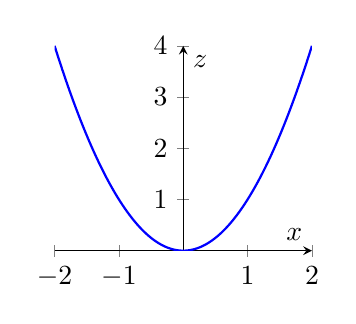
\begin{tikzpicture}
		\begin{axis}[
				axis lines=center,
				xlabel={$x$},
				ylabel={$z$},
				domain=-2:2,
				samples=100,
				width=0.4\textwidth,
			]
			\addplot[blue, thick] {x^2};
		\end{axis}
	\end{tikzpicture}
	\qquad
	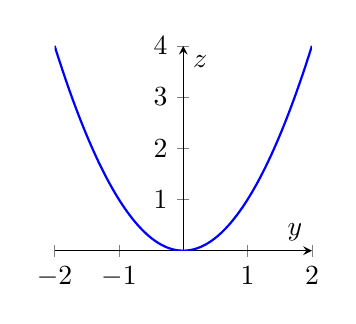
\begin{tikzpicture}
		\begin{axis}[
				axis lines=center,
				xlabel={$y$},
				ylabel={$z$},
				domain=-2:2,
				samples=100,
				width=0.4\textwidth,
			]
			\addplot[blue, thick] {x^2};
		\end{axis}
	\end{tikzpicture}
\end{center}

Alles in allem erwartet man somit bei K=(0,0) ein lokales Minimum.
Allerdings liegt ein Sattelpunkt vor!

% \begin{center}
% \begin{tikzpicture}
%     \begin{axis}[
%         view={30}{40},
%         axis lines=center,
%         xlabel={$x$},
%         ylabel={$y$},
%         zlabel={$z$},
%         domain=-3:3,
%         y domain=-3:3,
%         samples=30,
%         colormap/cool,
%         zmax=4,
%         zmin = -2,
%         clip mode=individual
%     ]
%         \addplot3[surf, opacity=0.7] {x^2 + y^2 + 4*x*y};

%          % xy-ebene
%         \addplot3[surf, opacity=0.25, colormap/blackwhite] 
%             coordinates {
%                 (-2, -2, 0) (-2, 2, 0) (2, -2, 0) (2, 2, 0)
%             };


%     \end{axis}
% \end{tikzpicture}
% \end{center}

\begin{center}
	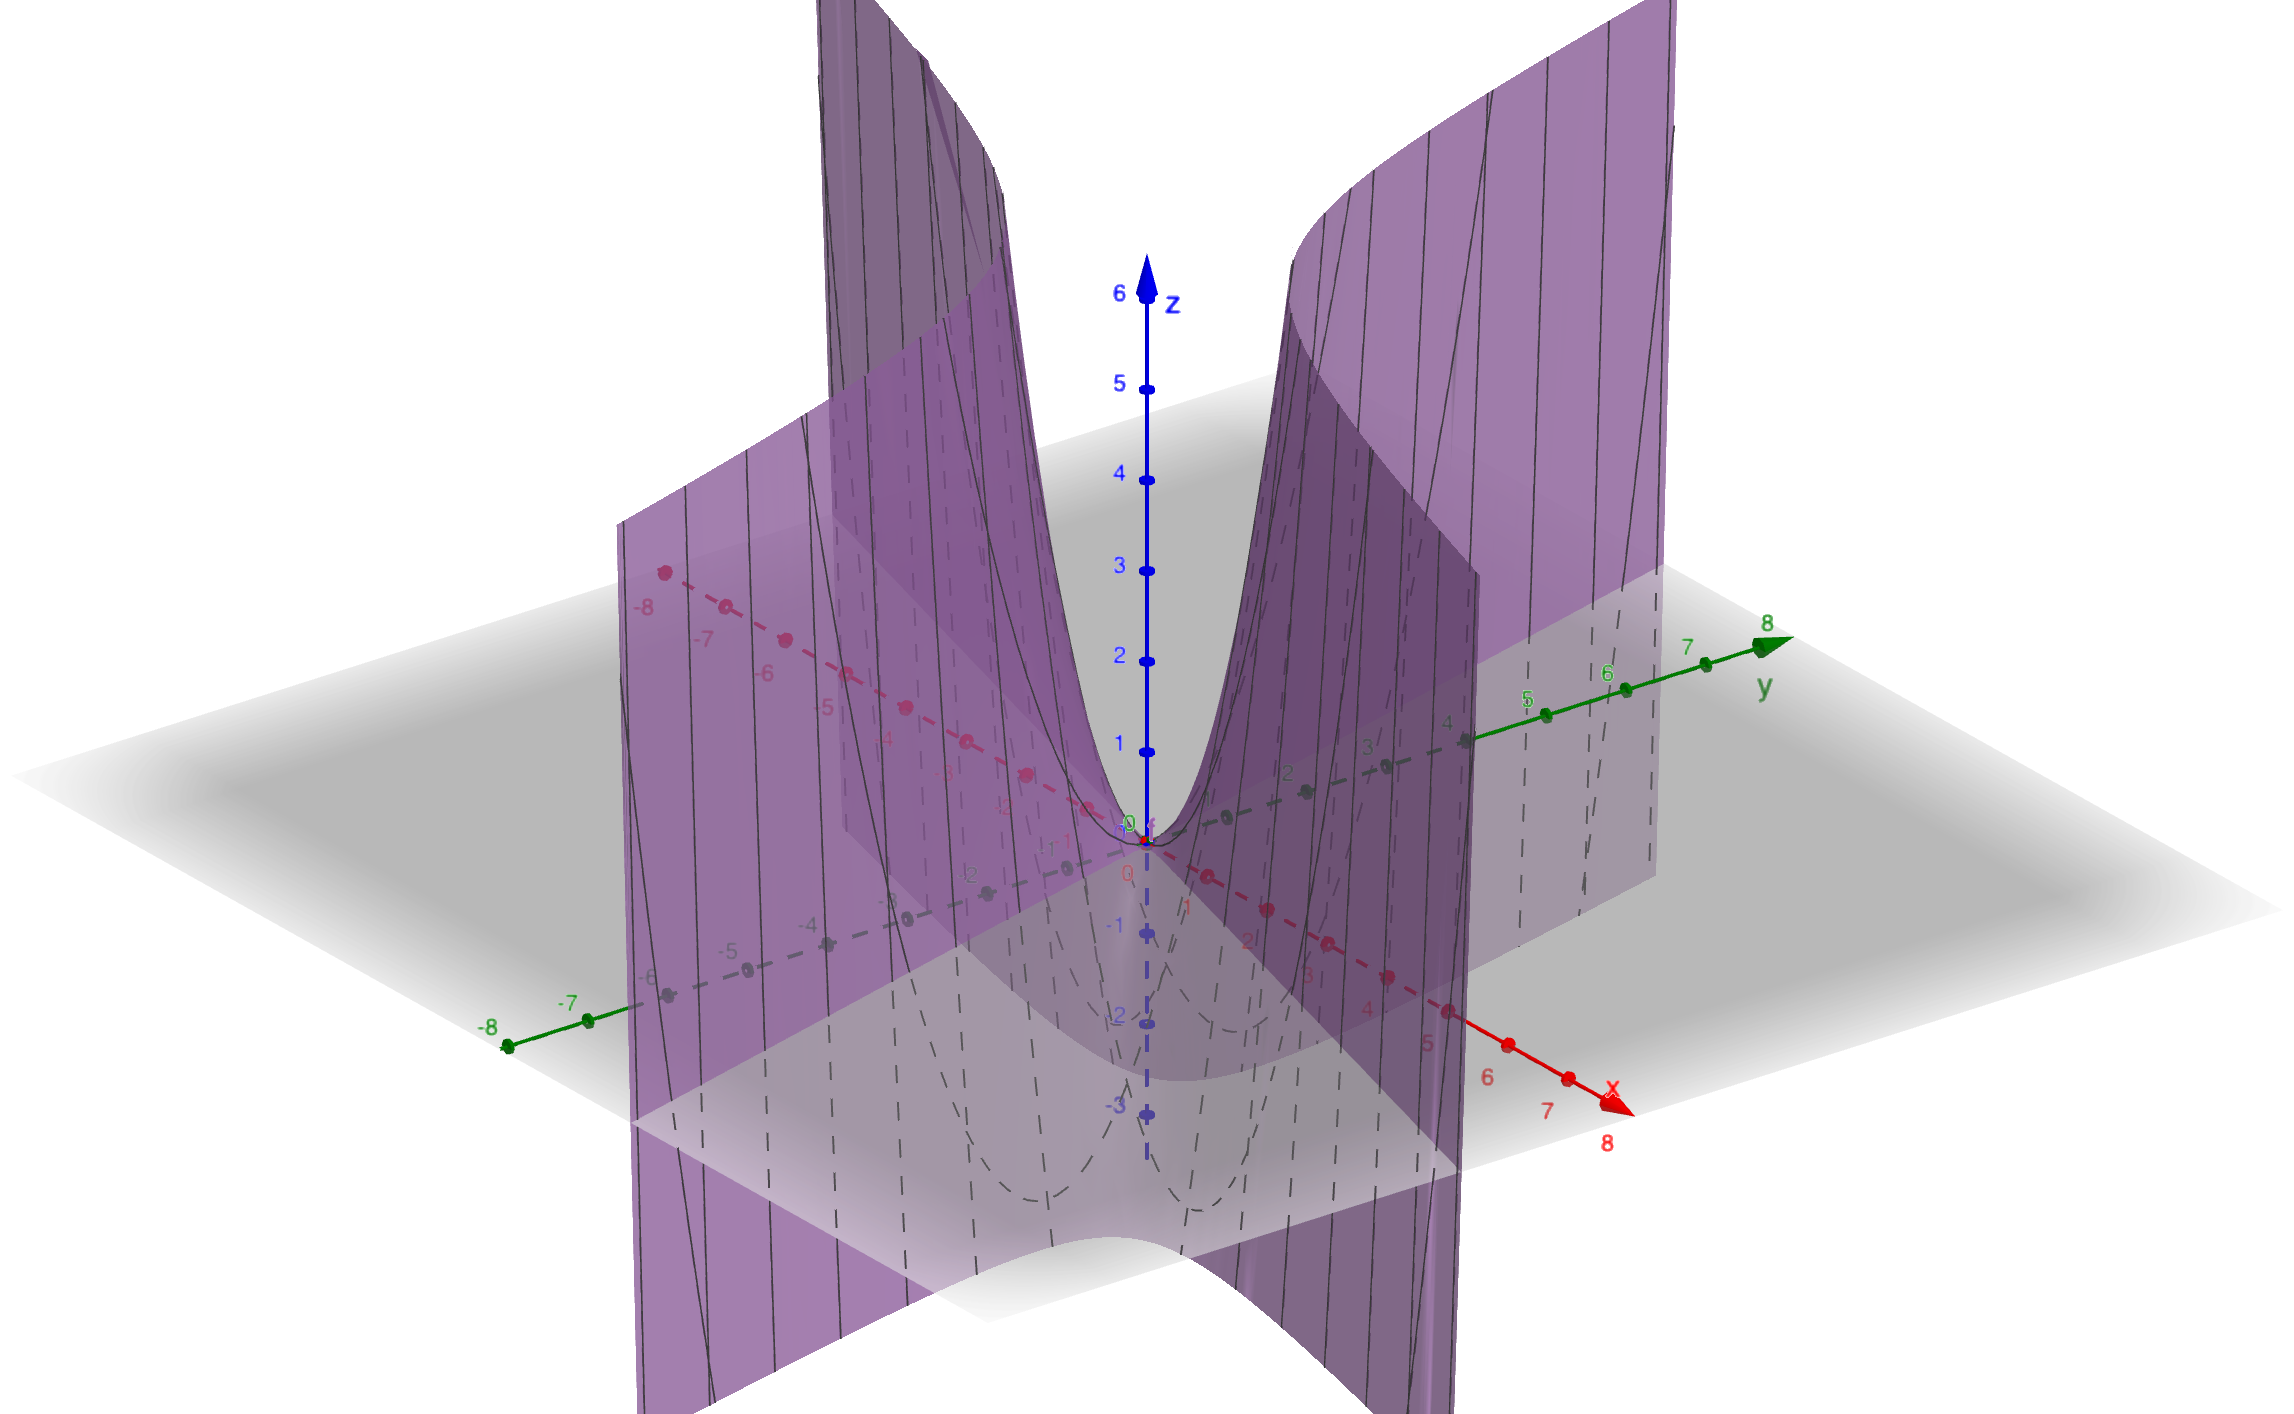
\includegraphics[width = 0.8 \textwidth]{media/introKriterien.png}
\end{center}



Betrachtet man den Graphen, so erkennt man das Problem: Die Schnittkurven in \(x\)- und \(y\)-Richtung weisen in der Tat ein lokales Minimum auf. Schneidet man den Graphen jedoch entlang einer Winkelhalbierenden der beiden Achsen, so hat die entsprechende Schnittkurve an der Stelle \((0,0)\) ein lokales Maximum.

Das kann auch rechnerisch bestätigt werden: Für die Richtungsableitung in Richtung \(\vec{v}=\begin{pmatrix} 1 \\ -1 \end{pmatrix}\) gilt
\[
	\frac{\partial f}{\partial \vec{v}}(x, y) =\left\langle \vec\nabla f(x,y) , \begin{pmatrix} 1 \\ -1 \end{pmatrix} \right\rangle = -2x + 2y
\]
Somit gilt \(\frac{\partial f}{\partial \vec{v}}(0,0) = 0\). Das widerspiegelt die Tatsache, dass die Schnittkurve in diese Richtung an der Stelle \((0,0)\) eine horizontale Tangente aufweist. Wie steht es aber mit der zweiten Ableitung in diese Richtung? Dazu berechnen wir die Richtungsableitung in Richtung \(\vec{v}=\begin{pmatrix} 1 \\ -1 \end{pmatrix}\) der Funktion \(z = -2x + 2y\):
\[
	\frac{\partial \left( -2x + 2y \right)}{\partial \vec{v}}  = \left\langle \vec \nabla \left( -2x + 2y \right) , \begin{pmatrix} 1 \\ -1 \end{pmatrix} \right\rangle = \left\langle \begin{pmatrix} -2 \\ 2 \end{pmatrix}, \begin{pmatrix} 1 \\ -1 \end{pmatrix} \right\rangle = -4.
\]
In Richtung \(\vec{v}=\begin{pmatrix} 1 \\ -1 \end{pmatrix}\) ist die zweite Ableitung negativ! Damit weist die Schnittkurve in diese Richtung ein lokales Maximum auf!


\subsubsection*{Fazit}
Damit ein lokales Minimum vorliegt, muss die zweite Richtungsableitung in \textbf{jede} Richtung positiv sein! Die Richtungsableitungen zweiter Ordnung lassen sich einfach mit der Hesse-Matrix berechnen. Betrachten Sie dazu die folgende Lernaufgabe:

\begin{LA}
	{}{}
	\textbf{Ziel:} Nachvollziehen, dass die zweifache Ableitung der Funktion \(f\) in einer bestimmten Richtung \(\vec{v}\) das gleiche ist wie das Skalarprodukt \(\langle \vec{v} ,\, H \vec{v} \rangle\), wobei \(H\) die Hesse-Matrix von \(f\) ist.

	\textbf{Aufgabe:} Sei zunächst \(f(x,y) = x^3y - xy^2\).
	\begin{enumerate}
		\item Berechnen Sie \(\vec{\nabla} f(x,y)\) und \(H(x,y)\).
		\item Sei \(\vec{v} = \begin{pmatrix} v_1 \\ v_2 \end{pmatrix}\). %mit \(|\vec{v}| = 1\)
		      Berechnen Sie die Richtungsableitung \(\frac{\partial f}{\partial \vec{v}}(x, y)\) in Abhängigkeit der beiden Einträge \(v_1\) und \(v_2\).
		\item \(\frac{\partial f}{\partial \vec{v}}(x, y)\) ist wieder eine Funktion von \(\mathbb{R}^2\) nach \(\mathbb{R}\). Berechnen Sie deren Gradient \(\vec{\nabla}\left(\frac{\partial f}{\partial \vec{v}}(x, y)\right)\).
		\item Berechnen Sie \(H(x,y) \cdot \vec{v}\) und zeigen Sie, dass \(H(x,y) \cdot \vec{v} = \vec\nabla\left(\frac{\partial f}{\partial \vec{v}}(x, y)\right)\) ist.
		\item Begründen Sie schliesslich, dass die zweite Ableitung in Richtung $\vec{v}$ \(\frac{\partial^2 f}{\partial \vec{v}^2} = \frac{\partial }{\partial \vec{v}}\left(\frac{\partial f}{\partial \vec{v}}(x, y)\right)\) das gleiche wie das Skalarprodukt \(\langle \vec{v} ,\, H \vec{v} \rangle\) ist.
		\item Führen Sie die gesamte Rechnung nochmals mit einer allgemeinen Funktion \(f(x,y)\) durch.
	\end{enumerate}
\end{LA}


\clearpage

\begin{satz}
	{Richtungsableitung zweiter Ordnung}{}
	Sei \(f(x,y)\) eine zweimal differenzierbare Funktion. Sei \(H(x,y)\) die Hesse-Matrix der Funktion und sei \(\vec{v} \in \mathbb{R}^2\). Dann gilt für die zweite Ableitung von \(f\) in Richtung \(\vec{v}\):
	\[
		\frac{\partial^2 f}{\partial \vec{v}^2} = \langle \vec{v} ,\, H \vec{v} \rangle.
	\]
\end{satz}

\begin{proof}


	Sei \(\vec{v} = \begin{pmatrix} v_1 \\ v_2 \end{pmatrix}\). Dann gilt für die Richtungsableitung
	\[
		\frac{\partial f}{\partial \vec{v}}(x, y) = \left\langle \vec\nabla f(x,y) ,\, \vec{v} \right\rangle= \frac{\partial f}{\partial x}(x,y) \cdot v_1 + \frac{\partial f}{\partial y}(x,y) \cdot v_2.
	\]
	Der Gradient dieser Richtungsableitung ist
	\[
		\vec\nabla\left(\frac{\partial f}{\partial \vec{v}}(x, y)\right) =
		\begin{pmatrix}
			\frac{\partial^2 f}{\partial x^2}(x,y) \cdot v_1 + \frac{\partial^2 f}{\partial x \partial y}(x,y) \cdot v_2 \\
			\frac{\partial^2 f}{\partial y \partial x}(x,y) \cdot v_1 + \frac{\partial^2 f}{\partial y^2}(x,y) \cdot v_2
		\end{pmatrix}
		=
		\begin{pmatrix}
			\frac{\partial^2 f}{\partial x^2}(x,y)          & \frac{\partial^2 f}{\partial x \partial y}(x,y) \\
			\frac{\partial^2 f}{\partial y \partial x}(x,y) & \frac{\partial^2 f}{\partial y^2}(x,y)
		\end{pmatrix}
		\cdot
		\begin{pmatrix}
			v_1 \\ v_2
		\end{pmatrix}
		= H \vec{v}.
	\]
	Für die zweite Ableitung von \(f\) in Richtung \(\vec{v}\) gilt damit:
	\[
		\frac{\partial^2 f}{\partial \vec{v}^2}  = \left\langle \vec{v} , \vec\nabla\left(\frac{\partial f}{\partial \vec{v}}(x, y)\right) \right\rangle = \left\langle \vec{v} , H \vec{v} \right\rangle.
	\]

\end{proof}

Wenn also die Matrix \(H\) die Eigenschaft hat, dass \(\langle \vec{v} ,\, H \vec{v} \rangle > 0\) für alle \(\vec{v} \in \mathbb{R}^2\), dann sind alle Richtungsableitungen zweiter Ordnung positiv. Solche Matrizen haben einen speziellen Namen:

\begin{definition}
	{Positive Definitheit}{}
	Eine Matrix \(H\) heisst positiv definit, wenn für alle \(\vec{v} \in \mathbb{R}^2\) gilt:
	\[
		\langle \vec{v} ,\, H \vec{v} \rangle > 0.
	\]
	Eine Matrix \(H\) heisst negativ definit, wenn für alle \(\vec{v} \in \mathbb{R}^2\) gilt:
	\[
		\langle \vec{v} ,\, H \vec{v} \rangle < 0.
	\]
	Eine Matrix \(H\) heisst indefinit, wenn es \(\vec{v} \in \mathbb{R}^2\) gibt, so dass \(\langle \vec{v} ,\, H \vec{v} \rangle > 0\) und \(\vec{w} \in \mathbb{R}^2\) so dass \(\vec{w} \cdot H \vec{w} < 0\).

\end{definition}

Wenn die Funktion \(f(x,y)\) zweimal stetig differenzierbar ist, ist die Hesse-Matrix eine symmetrische \(2 \times 2\)-Matrix. Für solche lässt sich die Definitheit leicht erkennen. Es gilt:
\begin{satz}
	{Kriterium für Definitheit}{}
	Eine symmetrische Matrix \(H\) ist genau dann positiv definit, wenn \(\det(H) > 0\) und \(h_{11} > 0\). Analog ist eine symmetrische Matrix \(H\) genau dann negativ definit, wenn \(\det(H) > 0\) und \(h_{11} < 0\). Falls \(\det(H) < 0\), ist \(H\) indefinit.
\end{satz}

Beweis: siehe nächstes Kapitel\dots



Zusammengefasst erhalten wir die folgenden einigermassen handlichen Kriterien, um festzustellen, welche Art kritischer Punkt vorliegt:
\begin{satz}
	{Klassifikation der kritischen Punkte}{}
	Sei \(f(x,y)\) eine zweimal stetig differenzierbare Funktion. Sei \(K = (x_0,y_0)\) eine kritische Stelle von \(f\) und sei \(H(K)\) die Hesse-Matrix an dieser Stelle. Dann gilt:
	\begin{enumerate}
		\item Ist \(\det(H(K)) > 0\) und \(h_{11} > 0\), so liegt an der Stelle \(K\) ein lokales Minimum vor.
		\item Ist \(\det(H(K)) > 0\) und \(h_{11} < 0\), so liegt an der Stelle \(K\) ein lokales Maximum vor.
		\item Ist \(\det(H(K)) < 0\), so liegt an der Stelle \(K\) ein Sattelpunkt vor.
	\end{enumerate}
\end{satz}

\begin{ueb}
	{}{}

	\begin{enumerate}
		\item Betrachten Sie nochmals die Funktion \(f(x,y) = x^3 + xy^2 - x\). Der Gradient und die kritischen Stellen haben wir in \Cref{bsp:kritischePunkte2} bereits ermittelt:
		      \[
			      \nabla f(x,y) = \begin{pmatrix}
				      3x^2 + y^2 - 1 \\
				      2xy
			      \end{pmatrix}
		      \]
		      \[
			      K_1 = (0,1), \quad K_2 = (0,-1), \quad K_3 = \left(\frac{\sqrt{3}}{3}, 0\right), \quad K_4 = \left(-\frac{\sqrt{3}}{3}, 0\right)
		      \]
		      Bestimmen Sie die Art der kritischen Punkte.

		\item Bestimmen Sie die lokalen Extrema und Sattelpunkte der folgenden Funktionen:
		      \begin{enumerate}
			      \item \(f(x,y) = x^2 - y^2\)
			      \item \(h(x,y) = \frac{1}{y} - \frac{1}{x} - 4x + y\)
			      \item \(k(x,y) = 3 \ln(x) - xy^2 + 2(y-x)\)
			      \item \(l(x,y) = (x^2 - 2x)(y^2 - 2y)\)
			      \item \(m(x,y) = \frac{1}{2}x^2 - \frac{1}{3}y^3 - xy + x - y - 1\)
			      \item  \(g(x,y) = (x+y)^2\)
			      \item \(j(x,y) = (x-1)^3 + (y-1)^3 - 3(x-1)(y-1) + 1\) Hinweis: Ersetze \(x-1\) durch \(u\) und \(y-1\) durch \(v\).
		      \end{enumerate}

		\item Eine Seilerei produziert Hanfseile in Naturfarben und blaue Hanfseile. Die Anzahlen \(x_N\) und \(x_B\) verkaufter Seile jeder Art pro Stunde hängen dabei jeweils von den Preisen \(p_N\) und \(p_B\) beider Produktionsartikel ab:
		      \[
			      x_N = 8 - 2p_N + p_B, \quad x_B = 9 + 2p_N - 2p_B
		      \]
		      Die Kosten für die Produktion eines naturfarbenen Seils belaufen sich auf 2 CHF. Jene für ein blaues Seil liegen bei 3 CHF. Wie soll die Seilerei die Preise \(p_N\) und \(p_B\) ansetzen, damit die Gewinne möglichst hoch ausfallen?
	\end{enumerate}

\end{ueb}

\clearpage
\emph{Lösungen}
\begin{enumerate}
	\item

	      \begin{itemize}
		      \item An den Stellen \(K_1\) und \(K_2\) gibt es einen Sattelpunkt.
		      \item Bei \(K_3\) ein lokales Minimum.
		      \item Bei \(K_4\) ein lokales Maximum.
	      \end{itemize}

	\item
	      \begin{enumerate}
		      \item \[
			            S = (0,0,0)
		            \]

		      \item \[
			            S_1 = \left(\frac{1}{2}, 1, -2\right), \quad H = \left(\frac{1}{2}, -1, -6\right), \quad T = \left(-\frac{1}{2}, 1, 6\right), \quad S_2 = \left(-\frac{1}{2}, -1, 2\right)
		            \]
		      \item \[
			            S = (1, 1, 1), \quad T = (2, 2, 0)
		            \]

		      \item \[
			            S_1 = (0, 0, 0), \quad S_2 = (0, 2, 0), \quad S_3 = (2, 0, 0), \quad S_4 = (2, 2, 0), \quad H = (1, 1, 1)
		            \]

		      \item \[
			            S = \left(-1, 0, -\frac{3}{2}\right), \quad T = \left(-2, -1, -\frac{5}{3}\right)
		            \]
		      \item
		            \begin{itemize}
			            \item Da \(\det(H) = 0\) ist, lässt sich das auf herkömmliche Weise nicht bestimmen.
			            \item Offensichtlich sind aber alle Funktionswerte positiv ausser auf den Punkten mit \(y = -x\).
			            \item Es gibt also unendlich viele Tiefpunkte:
			                  \[
				                  T = (x, -x, 0)
			                  \]
		            \end{itemize}
		      \item \[
			            H = (1, 1, -1), \quad S = \left(\frac{1}{2}, 2, 1 - \ln(8)\right)
		            \]
	      \end{enumerate}

	\item
	      \begin{enumerate}
		      \item \[
			            G(p_N, p_B) = (p_N - 2)(8 - 2p_N + p_B) + (p_B - 3)(9 + 2p_N - 2p_B)
		            \]
		      \item Der Gewinn ist maximal für \(p_N = 9\) und \(p_B = 10\).
	      \end{enumerate}
\end{enumerate}


























\clearpage
\subsection{Beweis der Kriterien für Definitheit}
\label{sec:beweisKriterien}

In den Übungen haben Sie häufig die folgenden hinreichenden Bedingungen für die Definitheit von symmetrischen Matrizen verwendet:

\noindent\fbox{\parbox{\textwidth}{Eine symmetrische Matrix \(H\) ist genau dann positiv definit, wenn \(\det(H) > 0\) und \(h_{11} > 0\). \\
		Analog ist eine symmetrische Matrix \(H\) genau dann negativ definit, wenn \(\det(H) > 0\) und \(h_{11} < 0\). \\
		Falls \(\det(H) < 0\), ist \(H\) indefinit.}}

In diesem Abschnitt werden wir die erste der eingerahmten Aussagen beweisen. Die beiden anderen kann man ähnlich begründen.


Für den Beweis werden wir einige Vorkenntnisse aus der linearen Algebra und Vektorgeometrie aufgreifen:
\begin{itemize}
	\item Sei \(A\) eine \(2 \times 2\)-Matrix. Wenn ein Vektor \(\vec{v} \in \mathbb{R}^2\) und eine Zahl \(\lambda \in \mathbb{R}\) existieren, mit \(A\vec{v} = \lambda \vec{v}\), dann nennt man \(\vec{v}\) einen Eigenvektor der Matrix \(A\) zum Eigenwert \(\lambda\).
	\item Die Eigenwerte sind die Nullstellen des charakteristischen Polynoms \(\det(A - \lambda E)\).
	\item Eine \(2 \times 2\)-Matrix heisst diagonalisierbar, wenn sie zwei linear unabhängige Eigenvektoren hat.
	      % \item Das Skalarprodukt von zwei Vektoren, die den Winkel \(\varphi\) einschliessen, ist definiert als
	      % \[
	      % \langle \vec{a} , \, \vec{b} \rangle = |\vec{a}| \cdot |\vec{b}| \cdot \cos \varphi.
	      % \]
	\item Zwei Vektoren \(\vec{a}\) und \(\vec{b}\) stehen genau dann senkrecht aufeinander, wenn \(\langle \vec{a} , \, \vec{b} \rangle = 0\) ist.
	\item Sei \(\vec{a} = \begin{pmatrix} a_1 \\ a_2 \end{pmatrix}\) und \(\vec{b} = \begin{pmatrix} b_1 \\ b_2 \end{pmatrix}\) die Komponentendarstellung der Vektoren \(\vec{a}, \vec{b}\) bezüglich der Standardbasis. Dann gilt
	      \[
		      \langle \vec{a} , \, \vec{b} \rangle = a_1 b_1 + a_2 b_2.
	      \]
	\item Das Skalarprodukt ist bilinear. Das heisst, für alle \(\vec{v}_1, \vec{v}_2, \vec{v}_3, \vec{v}_4 \in \mathbb{R}^2\) und \(a, b, c, d \in \mathbb{R}\) gilt:
	      \[
		      \langle a\vec{v}_1 + b\vec{v}_2 , \,  c\vec{v}_3 + d\vec{v}_4 \rangle = ac \cdot\langle\vec{v}_1 , \vec{v}_3 \rangle + ad \cdot\langle \vec{v}_1 , \vec{v}_4\rangle + bc\cdot \langle \vec{v}_2 , \vec{v}_3\rangle + bd \cdot\langle \vec{v}_2 , \vec{v}_4\rangle.
	      \]
\end{itemize}




\clearpage
\begin{LA}
	{Beweis Teil 1}{beweisTeil1}

	Im Folgenden betrachten wir symmetrische $2 \times 2$ Matrizen der Form
	\[
		A = \begin{pmatrix}
			a & b \\
			b & c
		\end{pmatrix}, \quad a, b, c \in \mathbb{R},
	\]
	mit $\det(A) > 0$ und $a > 0$.

	\subsubsection*{Ziele}
	\begin{enumerate}
		\item Matrizen dieser Art sind immer diagonalisierbar.
		\item Beide Eigenwerte sind positiv.
	\end{enumerate}

	Für die folgenden Aufgaben nehmen wir zunächst an, dass $b \neq 0$ gilt.
	\begin{enumerate}
		\item Zeigen Sie, dass das charakteristische Polynom die Form \(p(\lambda) = \lambda^2 - (a+c)\lambda + ac - b^2\) hat.
		\item Bestimmen Sie die Diskriminante des charakteristischen Polynoms und zeigen Sie, dass diese ein Term der Form \(U^2 + V^2\) und damit immer positiv ist.
		      Daraus folgt, dass die Matrix immer zwei verschiedene Eigenwerte hat und somit diagonalisierbar ist.
	\end{enumerate}

	Daraus folgt, dass die Matrix immer zwei verschiedene Eigenwerte hat und somit diagonalisierbar ist. und somit haben wir das erste Ziel erreicht.

	Zum zweiten Ziel:

	Für die nächsten Fragen benötigen Sie den Satz von Vieta:

	Seien \(x_1\) und \(x_2\) die Lösungen der Gleichung \(x^2 + Bx + C = 0\). Dann gilt:
	\[
		x_1 \cdot x_2 = C \quad \text{und} \quad x_1 + x_2 = -B.
	\]

	\begin{enumerate}[resume]
		\item Seien \(\lambda_1\) und \(\lambda_2\) die beiden Eigenwerte der Matrix \(A\). Zeigen Sie mit dem Satz von Vieta, dass \(\lambda_1 \cdot \lambda_2 = \det(A)\) ist.

		      Weil wir Matrizen mit \(\det(A) > 0\) betrachten, folgt daraus, dass die beiden Eigenwerte das gleiche Vorzeichen haben!
		\item Sei weiter \(\det(A) > 0\) und \(a > 0\):
		      \begin{enumerate}
			      \item Zeigen Sie zunächst, dass dann auch \(c > 0\) sein muss.
			      \item Zeigen Sie anschliessend mit dem Satz von Vieta, dass beide Eigenwerte der Matrix positiv sind.
		      \end{enumerate}
		\item Zusatz: Begründen Sie, wieso die beiden unter «Ziele» aufgeführten Aussagen auch stimmen, wenn \(b = 0\) ist.
	\end{enumerate}


\end{LA}

\clearpage

\begin{LA}
	{Beweis Teil 2}{beweisTEil2}
	\noindent Im Folgenden betrachten wir symmetrische Matrizen, also solche der Form
	\[
		A = \begin{pmatrix}
			a & b \\
			b & c
		\end{pmatrix}, \quad a, b, c \in \mathbb{R},
	\]
	mit zwei reellen, unterschiedlichen Eigenwerten \(\lambda_1 \neq \lambda_2\).

	\subsubsection*{Ziel}
	Die Eigenvektoren solcher Matrizen stehen senkrecht aufeinander.

	\begin{enumerate}
		\item Seien \(\vec{u} = \begin{pmatrix} u_1 \\ u_2 \end{pmatrix}\) und \(\vec{w} = \begin{pmatrix} w_1 \\ w_2 \end{pmatrix}\) zwei beliebige Vektoren. Zeigen Sie, dass
		      \[
			      \langle A \vec{u}, \vec{w} \rangle = \langle \vec{u}, A \vec{w} \rangle,
		      \]
		      wobei \(\langle \cdot, \cdot \rangle\) das Skalarprodukt bezeichnet.\\
		      \textbf{Bemerkung:} Dies gilt nur für symmetrische Matrizen.

		\item Seien \(\vec{v}_1\) und \(\vec{v}_2\) die Eigenvektoren der Matrix zu den Eigenwerten \(\lambda_1 \neq \lambda_2\). Begründen Sie jedes Gleichheitszeichen in der folgenden Rechnung:
		      \[
			      \lambda_1 \langle \vec{v}_1, \vec{v}_2 \rangle = \langle \lambda_1 \vec{v}_1, \vec{v}_2 \rangle = \langle A \vec{v}_1, \vec{v}_2 \rangle = \langle \vec{v}_1, A \vec{v}_2 \rangle = \langle \vec{v}_1, \lambda_2 \vec{v}_2 \rangle = \lambda_2 \langle \vec{v}_1, \vec{v}_2 \rangle.
		      \]

		\item Vergleichen Sie den Term ganz links mit jenem ganz rechts in der Gleichung oben und begründen Sie damit, dass die Eigenvektoren senkrecht aufeinander stehen.
	\end{enumerate}
\end{LA}


\clearpage

\begin{LA}
	{Beweis Teil 3}{beweisTeil3}
	\noindent Im Folgenden betrachten wir symmetrische $2 \times 2$ Matrizen, die diagonalisierbar sind, lauter positive Eigenwerte haben und deren Eigenvektoren senkrecht aufeinander stehen.

	\subsubsection*{Ziel}
	Wir wollen zeigen, dass eine solche Matrix positiv definit ist.

	\begin{enumerate}
		\item Sei \(A = \frac{1}{5} \begin{pmatrix} 14 & 2 \\ 2 & 11 \end{pmatrix}\). Zeigen Sie, dass \(\vec{v}_1 = \begin{pmatrix} 1 \\ -2 \end{pmatrix}\) und \(\vec{v}_2 = \begin{pmatrix} 2 \\ 1 \end{pmatrix}\) Eigenvektoren der Matrix sind, und weisen Sie nach, dass diese Matrix alle in der Voraussetzung genannten Eigenschaften besitzt.

		\item Sei nun \(\vec{w}\) ein beliebiger Vektor in \(\mathbb{R}^2\). Da die beiden Eigenvektoren der Matrix \(A\) linear unabhängig sind, lässt sich jeder Vektor in \(\mathbb{R}^2\) als Linearkombination der beiden Eigenvektoren angeben. Es gibt also zwei Zahlen \(\alpha, \beta \in \mathbb{R}\), sodass
		      \[
			      \vec{w} = \alpha \cdot \vec{v}_1 + \beta \cdot \vec{v}_2.
		      \]

		      \begin{enumerate}
			      \item Zeigen Sie, dass \(A \vec{w} = 2\alpha \cdot \vec{v}_1 + 3\beta \cdot \vec{v}_2\) ist.

			      \item Verwenden Sie die Bilinearität des Skalarprodukts und zeigen Sie, dass
			            \[
				            \langle \vec{w}, A \vec{w} \rangle = 10\alpha^2 + 15\beta^2.
			            \]

			      \item Wie genau fliessen die Eigenwerte und die Komponenten der Eigenvektoren in die Rechnung oben ein? Oder anders gefragt: Wie setzen sich die Zahlen \(10\) und \(15\) zusammen?

			      \item Begründen Sie, wieso auch jede andere Matrix mit den in der Voraussetzung genannten Eigenschaften immer positiv definit ist.
		      \end{enumerate}
	\end{enumerate}
\end{LA}

\clearpage
\subsubsection*{Zusammenfassung der Ergebnisse}

Die folgenden Überlegungen gelten für eine Stelle \((x_0, y_0)\) mit \(\vec{\nabla} f(x_0, y_0) = \vec{0}\), \(\det(H(x_0, y_0)) > 0\) und \(\frac{\partial^2 f}{\partial x^2}(x_0, y_0) > 0\):
\begin{itemize}
	\item Aus \(\vec{\nabla} f(x_0, y_0) = \vec{0}\) folgt, dass die Richtungsableitung in jede Richtung \(\vec{v}\) Null ist, weil
	      \[
		      \frac{\partial f}{\partial\vec{v}} (x_0,y_0) = \langle \vec{\nabla} f(x_0, y_0), \vec{v} \rangle = \langle \vec{0}, \vec{v} \rangle = 0.
	      \]

	\item Für die zweifache Richtungsableitung von \(f\) in Richtung \(\vec{v}\) gilt:
	      \[
		      \frac{\partial^2 f}{\partial\vec{v}^2}  = \langle \vec{v}, H \vec{v} \rangle.
	      \]

	\item Aus \(\det(H(x_0, y_0)) > 0\) und \(\frac{\partial^2 f}{\partial x^2}(x_0, y_0) > 0\) folgt (Teile 1-3), dass die Matrix \(H(x_0, y_0)\) positiv definit ist, also dass für jeden Vektor \(\vec{v}\) gilt:
	      \[
		      \langle \vec{v}, H \vec{v} \rangle > 0.
	      \]

	\item Der Graph von \(f\) hat demnach in jede Richtung \(\vec{v} = \begin{pmatrix} v_1 \\ v_2 \end{pmatrix}\) ein lokales Minimum. Damit meint man:
	      \begin{itemize}
		      \item Die Funktion \(t \mapsto f((x_0, y_0) + t \cdot (v_1, v_2))\) hat für jede Wahl von \((v_1, v_2) \in \mathbb{R}^2\) an der Stelle \(t = 0\) ein lokales Minimum.
		      \item Schneidet man den Graphen von \(f\) mit einer beliebigen Ebene, die durch den Punkt \((x_0, y_0, 0)\), parallel zur \(z\)-Achse und parallel zu \(\vec{v}\) verläuft, so entsteht eine Schnittkurve, die unabhängig von der Wahl von \(\vec{v} \in \mathbb{R}^2\) an der Stelle \((x_0, y_0)\) ein lokales Minimum hat.
	      \end{itemize}

	\item Das Bild unten zeigt den Graphen einer Funktion und den Schnitt mit einer Ebene durch den Tiefpunkt parallel zur \(z\)-Achse:
\end{itemize}
\begin{center}
	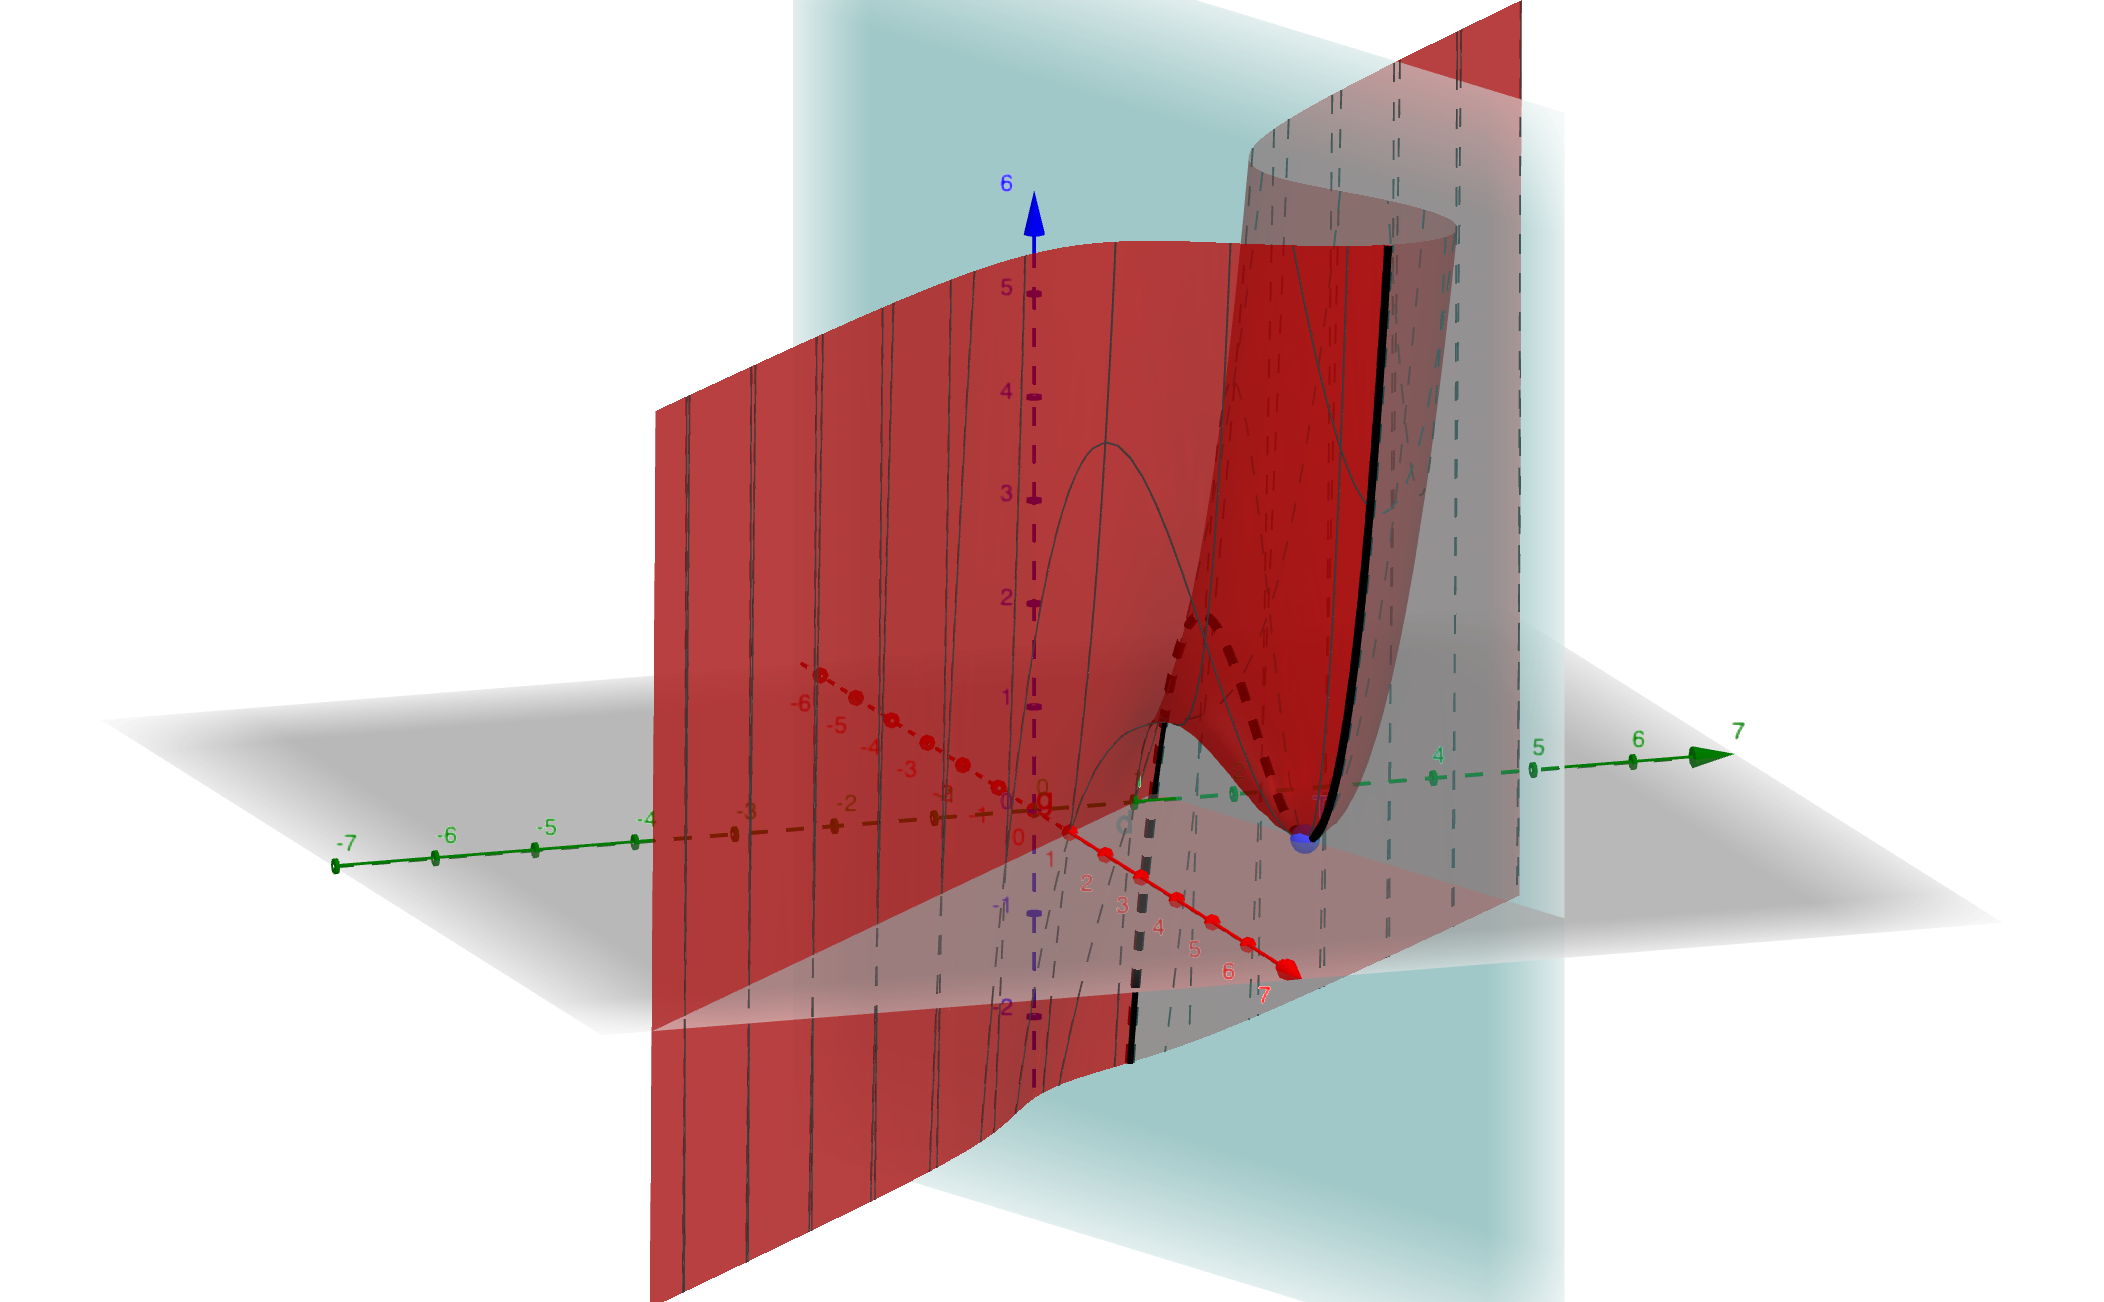
\includegraphics[width = 0.8\textwidth]{media/KriterienSchnitteneu.png}
\end{center}
